% jobs
% different p1, p2 shapes
% different Smith function shapes
% set defined on sphere or on projection?

%**************************************************************************
%
% # $Id: AWFE.Rnw,v 1.3 2007/03/15 22:52:05 js229 Exp $



\documentclass[a4paper]{article}


\title{
Edwards-Venn diagrams
}
\author{Jonathan Swinton}


\usepackage{float}
\usepackage{natbib}
\usepackage{mathptmx}
\usepackage{rotating} 
\usepackage[nodayofweek]{datetime}\longdate
\usepackage{hyperref}
\usepackage{c:/JonathanSwinton/r-devel/share/texmf/Sweave}
\begin{document}


\maketitle


Polar coordinates with longitude $\theta$ and latitude $\phi$. Arc distance
from the equator is $s$ and height above the equarorial plane is $h$.
\begin{eqnarray*}
s &=& r \frac{\phi}{2\pi}
\\
h &=& r \sin \phi
\end{eqnarray*}
Project down onto the equatorial plane (a polar stereographic projection).
\begin{eqnarray*}
\rho &=& \frac{\cos\phi}{1-\sin\phi} 2r
\\
x &=& \rho \cos \theta
\\
y &=& \rho \sin \theta
\end{eqnarray*}
A Mercator projection onto the (?) equatorial cylinder
\begin{eqnarray*}
x &=& r \cos \phi \cos \theta
\\
y &=& r \cos \phi \sin \theta
\end{eqnarray*}
\begin{eqnarray*}
x &=&  r theta
\\
y &=& h
\end{eqnarray*}

In a Mercator projection the Smith functions are
\begin{eqnarray*}
h &=& \frac{ \cos(2^{n-2} \theta)}{2^{n-2}}
\end{eqnarray*}

Let 
\begin{eqnarray*}
T_n &=& \frac{1}{2^n}\cos{2^n x}
\\
&=&  \frac{1}{2^n}\cos\frac{1}{2}{2^{n+1} x}
\\
2^{2n} T_n^2 &=& \frac{1}{2}\left( 1+ 2^{n+1}T_{n+1}\right)
\\
T_{n+1} &=& 2^{n} T_n^2 - \frac{1}{2^{n+1}}
\end{eqnarray*}
So $T_{n+1}=0$ when $T_n=\pm 2^{-n} 1/\sqrt(2)$; $2^nx=\pi/4+(p/2)2\pi$.




















\begin{figure}[H]\begin{center}
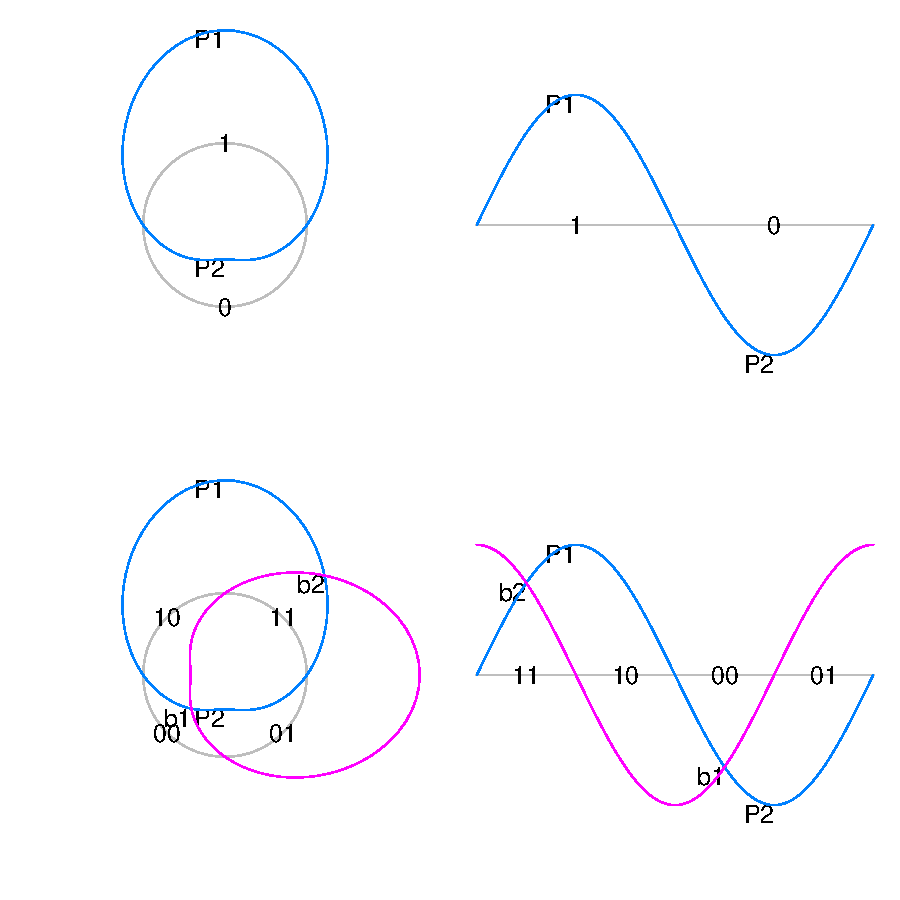
\includegraphics{Vennfig-rdovpspto2}
\caption{Additional nodes P1 and P2 introduced for n=1 and n=2 to avoid nasty edge condition s=0 to s=1
and to ensure no more than one directed edge between any pair of nodes.}
\end{center}\end{figure}

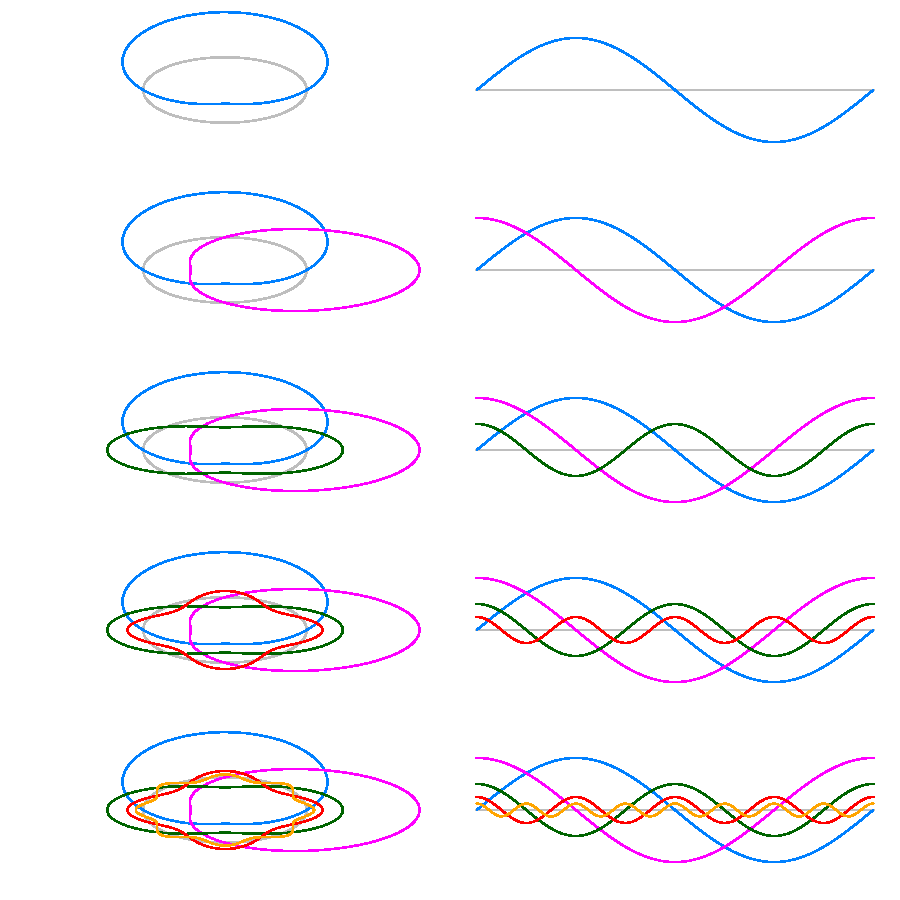
\includegraphics{Vennfig-rdovpsp}

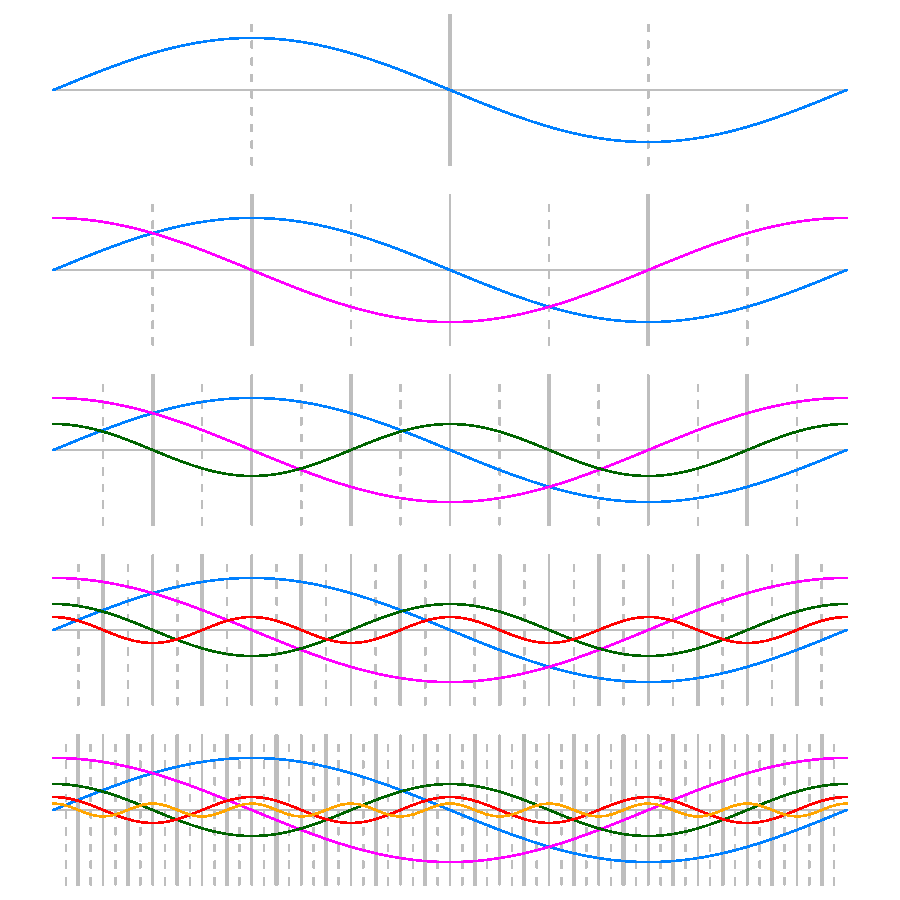
\includegraphics{Vennfig-rfdovpsp}


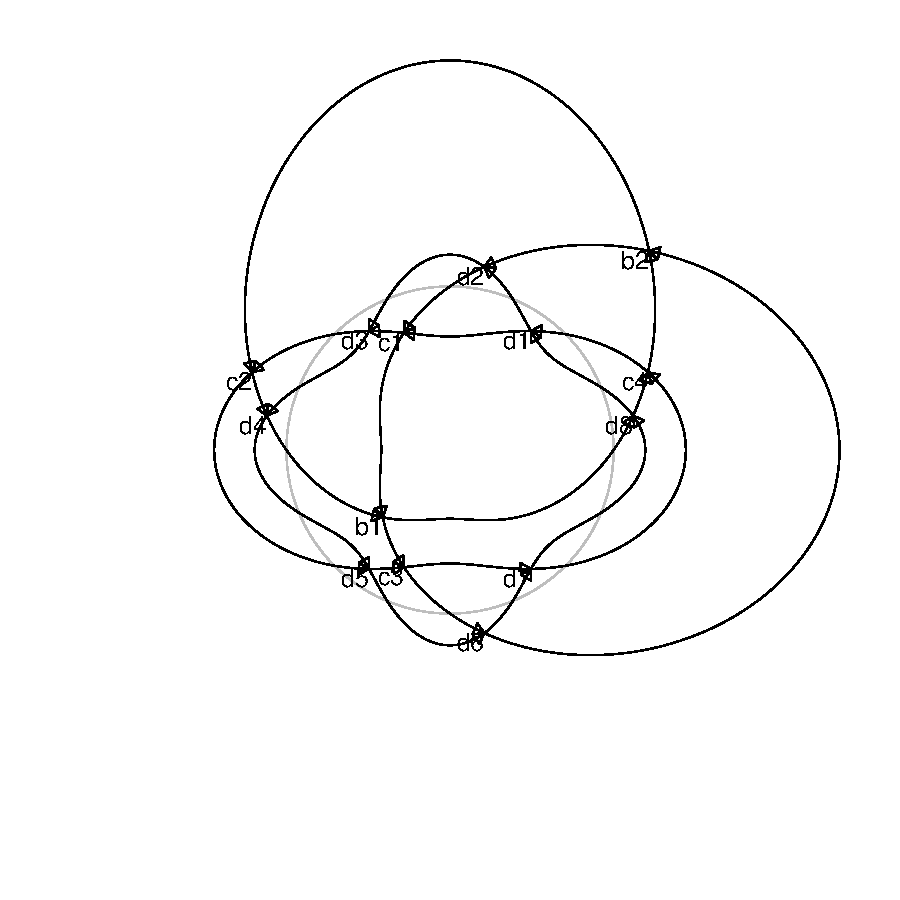
\includegraphics{Vennfig-rfdovpsp4}




\bibliographystyle{plain}
\bibliography{Venn}

\end{document}
